\documentclass[a4paper,11pt]{article}

\usepackage{wrapfig}
\usepackage{amsmath}
\usepackage{bm}
\usepackage{multicol}
\usepackage{pgfplots}
\usepackage{enumerate}
\usepackage{longtable}
\usepackage{rotating}
\usepackage{xcolor}
\usepackage{caption}
%\usepackage{minted}
\usepackage[most]{tcolorbox}
%Russian-specific packages
\usepackage[T2A]{fontenc}
\usepackage[utf8]{inputenc}
\usepackage[russian, english]{babel}
\usepackage{movie15}

\usepackage[left=2.5cm, right=1.5cm, vmargin=2.5cm]{geometry}
\usepackage[unicode, pdftex]{hyperref} % подключаем hyperref
\definecolor{linkcolor}{HTML}{111111} % цвет ссылок
\definecolor{urlcolor}{HTML}{799B03} % цвет гиперссылок

\hypersetup{pdfstartview=FitH,  linkcolor=linkcolor,urlcolor=urlcolor, colorlinks=true}

\usepackage{ragged2e}
\usepackage{hyperref}
\justifying

\begin{document}

\begin{titlepage}
  \center
  \textsc{\Large «Санкт-Петербургский политехнический \\ университет Петра Великого»}\\[0.5cm]
  \textsc{\large Институт компьютерных наук и технологий}\\
  \textsc{\large Высшая школа программной инженерии}\\[5.5cm]

  {
    \huge {Курсовая работа} \\[0.1cm]
    \Large {по дисциплине «Микропроцессорные системы»}
  } \\[4cm]

  \begin{multicols}{2}
  \begin{flushleft}
    {\Large Выполнили} \\[1.5mm] {\Large студенты гр. 3530904/80101}\\[2.0cm]
    {\Large Руководитель}
  \end{flushleft}
  \begin{flushright}
    \textcolor{white}{!}\\
    \Large {Пылаев Я. С.}\\
    \Large {Смирнов П. А.}\\
    \Large {Трофимов Ф. О.}\\[0.5cm]
    {\Large Круглов С. К.}
  \end{flushright}
  \end{multicols}

  \vspace{5cm}
  \centering
  \Large {
    Санкт-Петербург\\
    2020
  }
  \vfill
\end{titlepage}
\newpage

\def\contentsname{Содержание}
\begin{center}
  \tableofcontents
\end{center}
\newpage

\section{Задание}
\noindent Реализовать бытовую систему или устройство на основе процессора семейста ARM. Особенно важно сдлеать исследование стуртуры и возможностей аппаратуры. 
\section{Общее описание проектируемой системы}
\noindent \textbf{My-HomeCam-Security} - система контроля входа в умном доме.
\subsection{Сценарий использования}
\noindent Когда гость подходит к входной двери и нажимает на ней кнопку звонка (1), срабатывает распознавание лица (2) и фотография человека вместе с информацией о нем отправляется прямиком на мобильное устройство хозяина дома (3). Далее хозяин решает званный или нет гость стоит у него за дверью, нажимая соответствующую кнопку в приложении (4), и дверь в зависимости от этого решения открывается либо остается закрытой (5). Также владелец в любой момент может включить прямую трансляцию с камеры системы, тем самым наблюдая за входом в реальном времени. Общая схема работы системы представлена на \textit{Figure 1}.
\begin{center}
  \begin{figure}[h]
    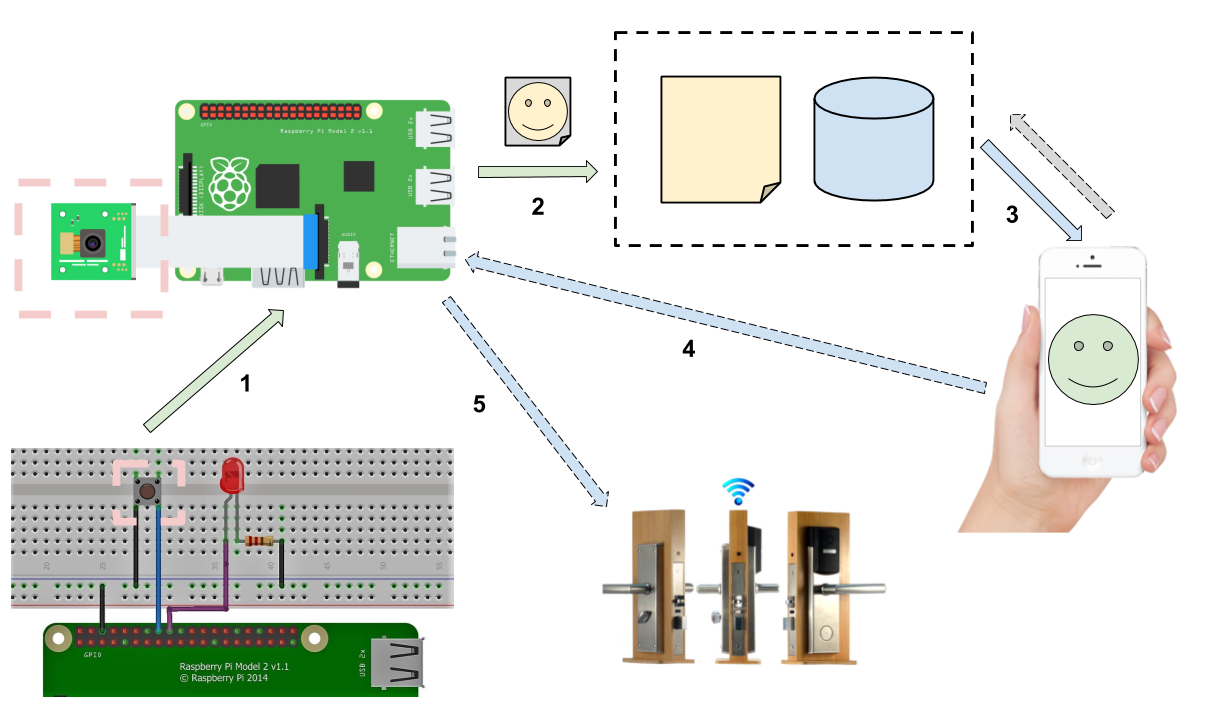
\includegraphics[scale=0.4]{images/Рисунок 1.png}
    \caption{Общая схема работы}
  \end{figure}
\end{center}

\subsection{Требования}
\noindent Для описанного сценария была выбрана следующая реализация:
\begin{itemize}
  \item Основынм аппаратным модулем является одноплатыный компьютер Raspberry Pi.
  \item Кнопка, световой индикатор и камера - непосредственно подключаются к "малинке".
  \item В качестве приложения для упарвления системой выбран формат бота Telegram.
  \item Язык программной реализации - Python.
\end{itemize}

\section{Аппаратная часть}
\subsection{Микрокомпьютер Raspberry Pi 3 Model B}
На устройстве установлен 64-х битный четырехъядерный процессор \textbf{ARM Cortex-A53} с тактовой частотой 1,2 ГГц на ядро в составе однокристальной платформы Broadcom BCM2837. Данный чип обеспечивает прирост производительности на 50–60% в сравнении с Raspberry Pi 2 и почти десятикратное преимущество перед первым Raspberry Pi. Благодаря этому компьютер обеспечивает ещё больше возможностей для «интернета вещей» и встраиваемых проектов.
Подробные харакатеристики предствлены на рисунке ниже.
\begin{center}
  \begin{figure}[h]
    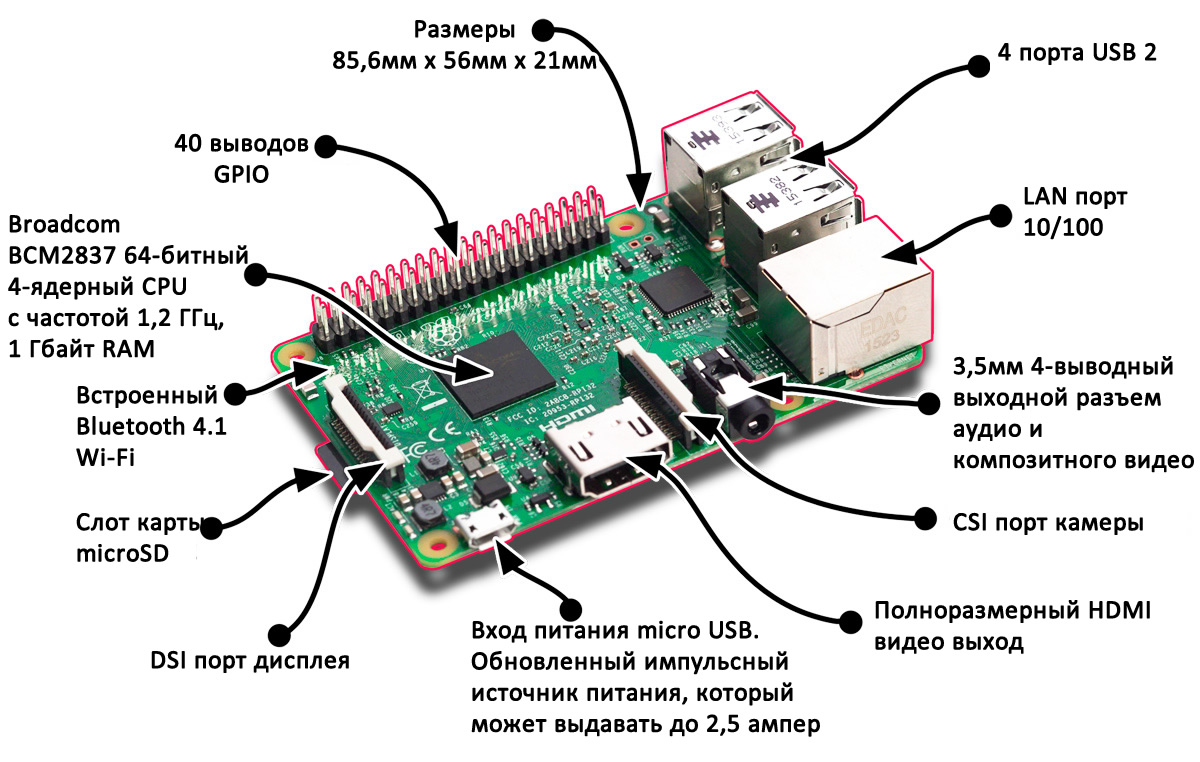
\includegraphics[scale=0.4]{images/pic_2.jpeg}
    \caption{Расположение компонентов на Raspberry Pi 3 Model B}
  \end{figure}
\end{center}

\subsection{Подключение периферийных устройств}
\noindent Для подключения монитора или телевизора используется композитный видеовыход или разъём HDMI. Разрешение варьируется от 640×350 (EGA) до 1920×1200 (WUXGA) для HDMI. Композитный выход работает в форматах PAL и NTSC. Raspberry Pi 3 Model B предоставляет 4 USB-порта, объединённых внутренним хабом. К ним, помимо прочего, можно подключить клавиатуру и мышь. \\

\noindent Для экономии ресурсов центрального процессора, Raspberry Pi предлагает подключения штатных модулей через 15-пиновые слоты:
\begin{itemize}
  \item CSI-2 — для подключения камеры по интерфейсу MIPI;
  \item DSI — для подключения штатного дисплея.
\end{itemize}
В качестве низкоуровневых интерфейсов доступны:
\begin{itemize}
  \item 40 портов ввода-вывода общего назначения;
  \item UART (Serial);
  \item I²C/TWI;
  \item SPI с селектором между двумя устройствами;
  \item пины питания: 3,3 В, 5 В и земля.
\end{itemize}
Для коммуникации на Raspberry Pi 3 Model B доступны интерфейсы:
\begin{itemize}
  \item Ethernet на 10/100 Мбит с выходом на стандартное гнездо 8P8C;
  \item Wi-Fi 802.11n и Bluetooth 4.1, обеспечиваемые микросхемой Broadcom BCM43438.
\end{itemize}

\subsection{Raspberry Pi Camera Module Rev 1.3}
\subsubsection{Описание камеры}
\begin{center}
  \begin{figure}[h]
    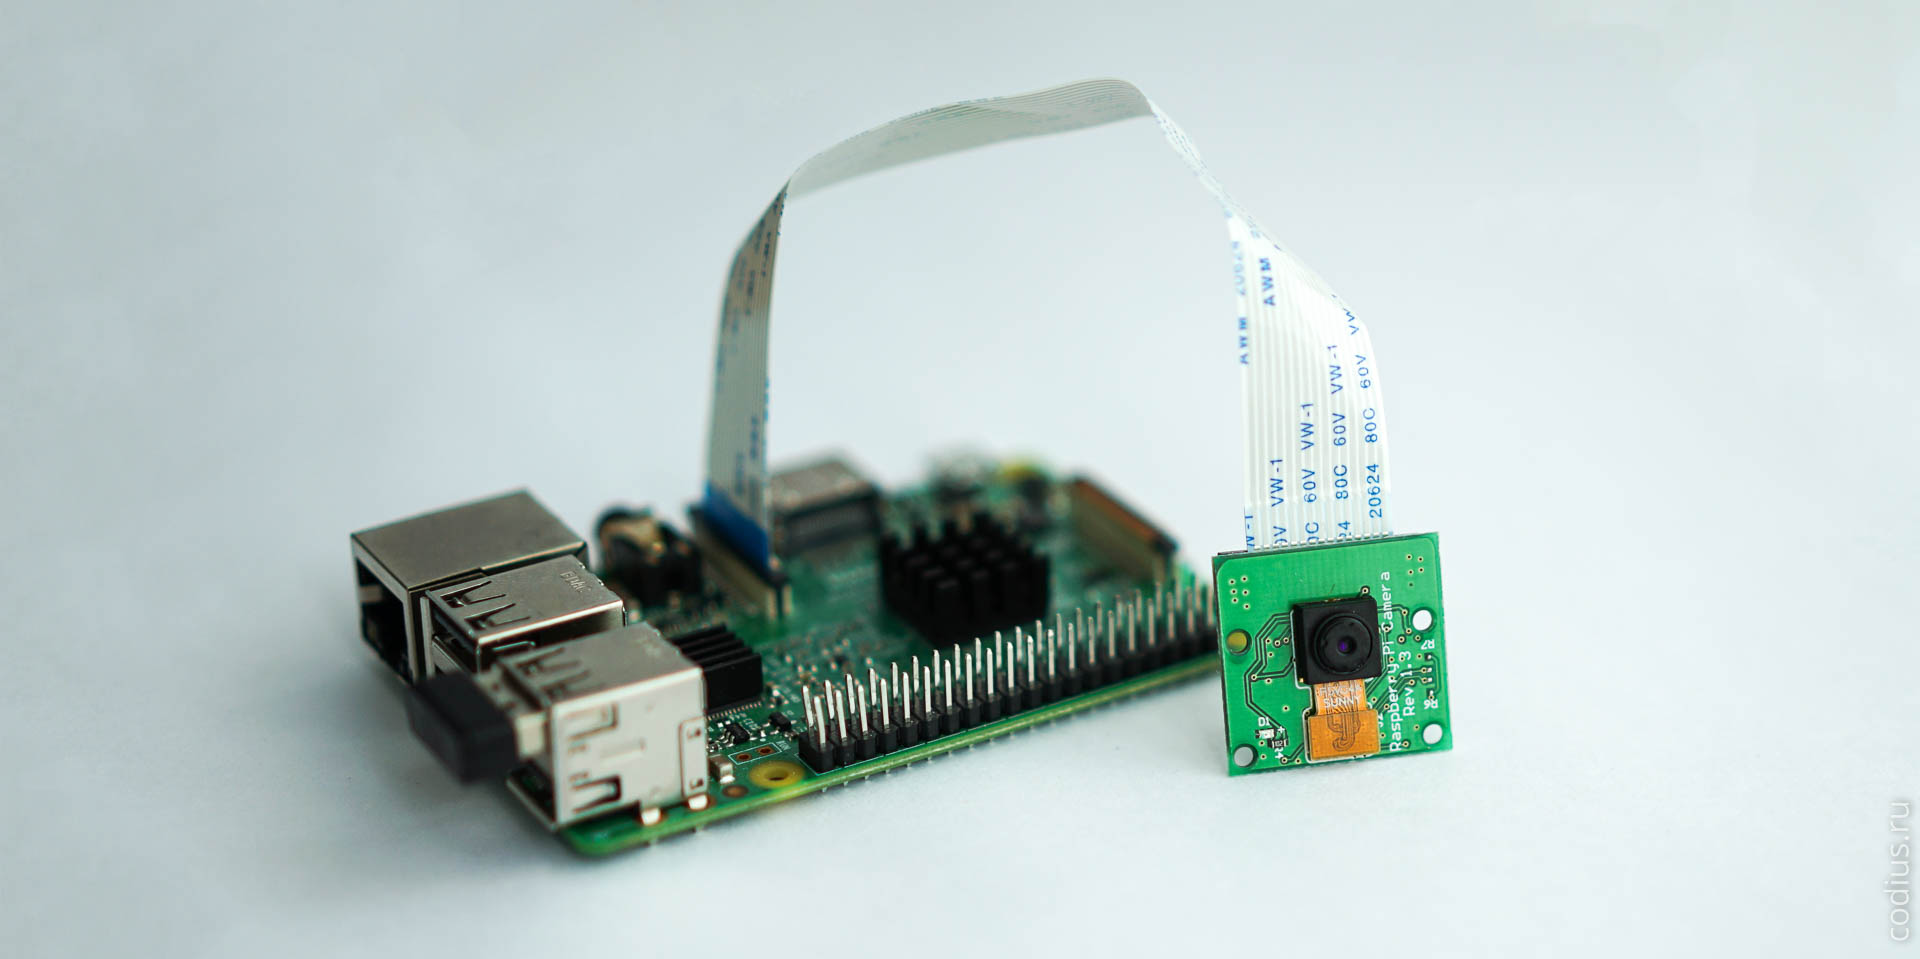
\includegraphics[scale=0.8]{images/pic_3.jpg}
    \caption{Raspberry Pi Camera Module Rev 1.3}
  \end{figure}
\end{center}
\noindent Камера Raspberry Pi подключается непосредственно к разъему CSI на Raspberry Pi. Она способен обеспечить качественное изображение с разрешением 5 МП или запись HD-видео 1080p со скоростью 30 кадров в секунду. Модуль камеры Raspberry Pi оснащен 5-мегапиксельным датчиком Omnivision 5647 в модуле фиксированной фокусировки. Модуль подключается к Raspberry Pi с помощью 15-контактного ленточного кабеля к специальному 15-контактному последовательному интерфейсу камеры MIPI (CSI), который был разработан специально для взаимодействия с камерами. Шина CSI способна обеспечивать чрезвычайно высокую скорость передачи данных и передает пиксельные данные напрямую процессору. Что касается неподвижных изображений, камера способна воспроизводить статические изображения 2592 x 1944 пикселей, а также поддерживает видео 1080p при 30 кадрах в секунду, 720p при 60 кадрах в секунду и 640x480p при 60/90 кадрах.\\

\subsubsection{Принципиальная схема}
\begin{center}
  \begin{figure}[h]
    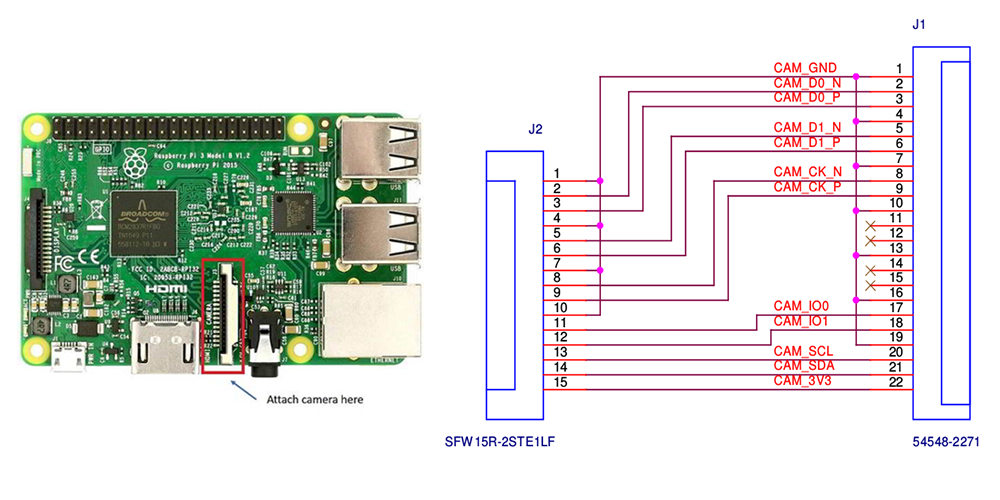
\includegraphics[scale=0.5]{images/pic_7.png}
    \caption{Подключение камеры в CSI порт}
  \end{figure}
\end{center}

\subsubsection{Технические характеристики}
\begin{itemize}
  \item  Размер: 25 × 24 × 9 mm
  \item Разрешение: 5 мегапикселей
  \item Видеорежимы: 1080p30, 720p60, 640×480p60/90	
  \item Сенсор: OmniVision OV5647	
  \item Разрешение сенсора: 2592 × 1944 пикселей	
  \item Отношение сигнал/шум: 36 дБ
  \item Фиксированный фокус: От 1 метра
  \item Фокусное расстояние: 3.60 мм
  \item Горизонтальное поле зрения: 53.5 градусов
  \item Вертикальное поле зрения: 41.4 градусов
  \item Рабочая температура: от -20 до +70 ºС
  \item Цвет: 24-Bit True color
  \item Структура пикселов: Байеровская
\end{itemize}

\subsubsection{Программные возможности}
\begin{itemize}
  \item Формат изображения: JPEG, GIF, BMP, PNG, YUV420
  \item Формат видео: raw h.264
  \item Эффекты: negative, solarise, posterize, whiteboard, blackboard, sketch, denoise, emboss, oilpaint, hatch, gpen, pastel, watercolour, film, blur, saturation
  \item Режимы экспозиции: auto, night, nightpreview, backlight, spotlight, sports, snow, beach, verylong, fixedfps, antishake, fireworks
  \item Режимы баланса белого: off, auto, sun, cloud, shade, tungsten, fluorescent, incandescent, flash, horizon
\end{itemize}

\subsection{Макетная плата MB102}

\begin{center}
  \begin{figure}[h]
    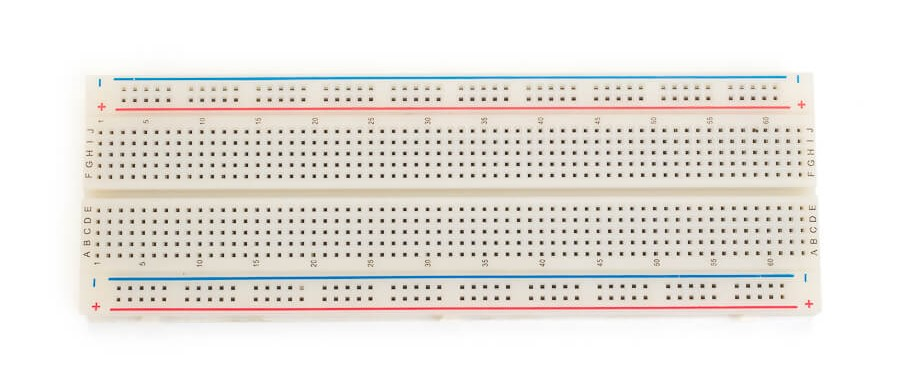
\includegraphics[scale=0.7]{images/pic_8.jpg}
    \caption{Макетная плата MB102}
  \end{figure}
\end{center}
\noindent Макетная плата, имеющая четыре пары рель для подключения питания и заземления позволяет создать функционирующий макет микросхемы. В платформе имеется 830 отверстий для простой установки контактов между различными элементами прототипируемого устройства. Центральное поле платформы имеет пять рядов контактов, в каждом из которых 126 отверстий. Еще два ряда по 100 контактов расположены по бокам макетной платы.
\subsubsection{Технические характеристики}
\begin{itemize}
  \item Размеры платформы: 165 х 55 х 8,5 mm
  \item Вес: 54 г
  \item Максимальное сопротивление контактов: 100 мОм
  \item Сопротивление изолятора: 1000 мОм
  \item Диапазон рабочих температур: от -20 до 80 ºС
  \item Максимально допустимая кратковременная температура: +150ºС
  \item Количество контактных отверстий: 830
\end{itemize}

\subsubsection{Приницпиальная схема}
\begin{center}
  \begin{figure}[h]
    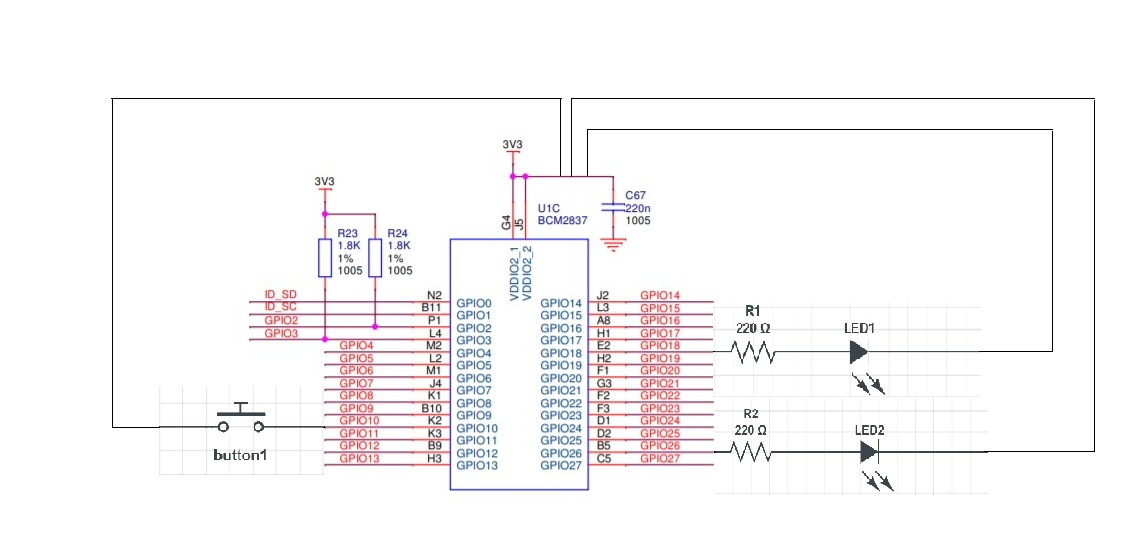
\includegraphics[scale=0.4]{images/рис_12.jpg}
    \caption{Подключение кнопки и светодиодов}
  \end{figure}
\end{center}

\section{Интерфейсы}
\subsection{GPIO}
В нашем проекте для работы кнопки и светодиодов используется интерфейс GPIO (General Purpose Inputs/Outputs) – выводы общего назначения. GPIO — это группа контактов, которыми можно управлять программным образом. Причем управлять  можно и простыми процессами, например, включение/выключение светодиода, и весьма сложными — обмен данными с периферийными устройствами по специализированным протоколам.

  \begin{figure}[h!]
    \begin{center}
    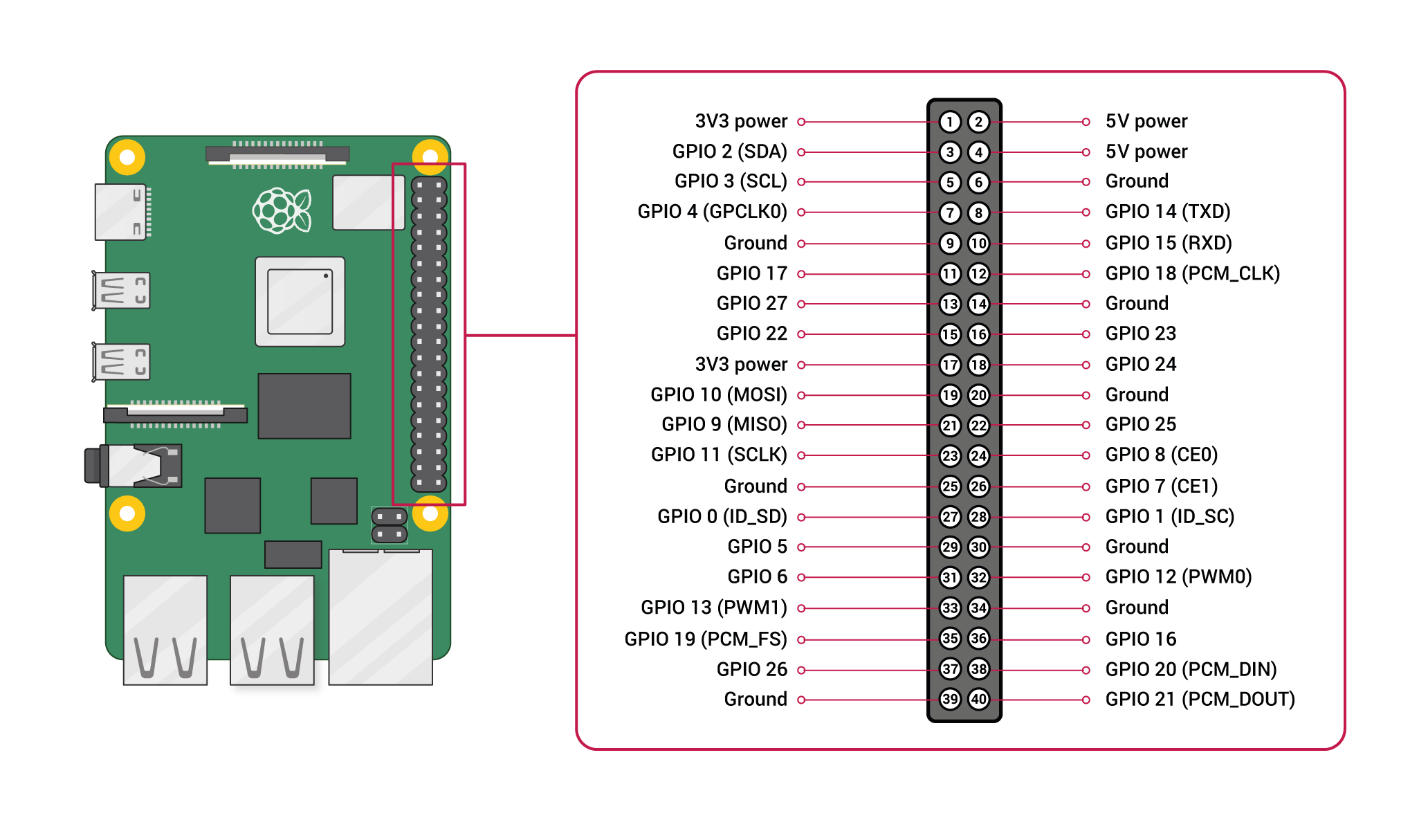
\includegraphics[scale=0.25]{images/рис_9.png}
    \caption{Распиновка GPIO выходов}
  \end{center}
  \end{figure}

\newpage
\noindent В терминах цифровой электроники управлять — значит менять на выводе уровень напряжения. Другими словами, все что мы можем сделать с помощью программы — это соединить желаемый вывод либо с контактом питания (+$3.3$ В), либо с землей (Gnd). Изобразим это на принципиальной схеме: \\
  
\begin{figure}[h!]
    \begin{center}
      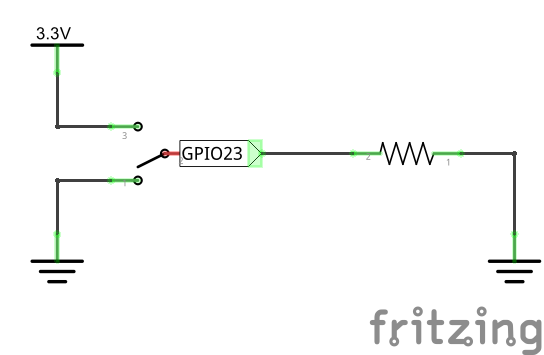
\includegraphics[scale=0.7]{images/рис_11.png}
      \caption{Управление GPIO выходом}
    \end{center}
  \end{figure}

\noindent На схеме имеется резистор, соединенный справа с землей — это наша нагрузка. Вместо резистора может быть светодиод, реле, зуммер, и т.п. Вывод GPIO23 и переключатель прямо за ним символизируют внутреннее устройство каждого вывода общего назначения.

\subsubsection{Учет падения напряжения}
\begin{itemize}
  \item Рабочее напряжение светодиода - $2 - 2.2$ В,
  \item Потребляемый ток светодиода - $20$ мА,
  \item Выходной ток Raspberry Pi - $3.3$ В. 
\end{itemize}
\begin{gather}
  3.3 V - 2 V = 1.3 V, \\
  R = \dfrac{U}{I} = \dfrac{1.3 V}{0.02 A} = 65 Om
\end{gather}
\noindent Настолько нужно понизить напряжение и, получив необходимое сопротивление резистора $65$ Ом, взяли ближайший доступный резистор на $220$ Ом.

\subsubsection{PULL-UP / PULL-DOWN резисторы}
Для установки начального состояния GPIO выхода при подключении кнопки используется внутренний подтягивающий резистор Raspberry Pi. Имеется два режима состояния, которые можно задавать программно:
\begin{itemize}
  \item Подтягивает пин к напряжению 3,3V\begin{verbatim}
    GPIO.setup(1, GPIO.IN, pull_up_down=GPIO.PUD_UP)
  \end{verbatim} 
  \item Подтягивает пин к земле
  \begin{verbatim}
    GPIO.setup(1, GPIO.IN, pull_up_down=GPIO.PUD_DOWN) 
  \end{verbatim}
\end{itemize}

\noindent В нашем проекте пин изначально подтянут к напряжению, и, пока кнопка не нажата, GPIO вход считывает значение TRUE, но при опускании кнопки напряжение на входе понижается и значение меняется на FALSE. \\

\begin{figure}[h!]
  \begin{center}
    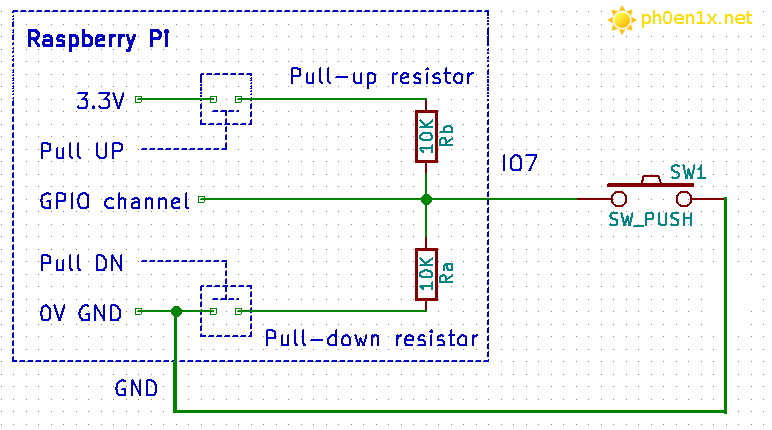
\includegraphics[scale=0.55]{images/рис_10.png}
  \caption{Подключение кнопки с использованием подтягивающего резистора}
  \end{center}
\end{figure}

\subsection{CSI}
\noindent Для начала отвтетим на вопрос, почему мы решили подключить камеру в CSI порт, а не через USB 3.0. Для нашей системы требуется высокая скорость анализа изображений, так как мы и так имеем некоторый замедлитель в виде распознавания лица, а Camera Serial Interface пин как раз обеспечивает поступакние изображение с камеры сразу на графический процессор, без промежуточной обработки, как в случае с USB 3.0. Грубо говоря CSI и создан для подобных задач. \\

\noindent Формирование изображения на матрице камеры происходит при помощи фильтра Байера. Это двумерный массив цветных фильтров, которыми накрыты фотодиоды фотоматрицы. Фильтр состоит из $25\%$ красных элементов, $25\%$ синих и $50\%$ зеленых элементов.
  \begin{figure}[h!]
    \begin{center}
      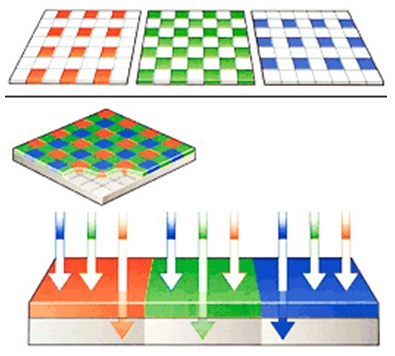
\includegraphics[scale=0.7]{images/рис_13.jpg}
    \caption{Фильр Байера}
    \end{center}
  \end{figure}
\newpage
\noindent Далее на рисунке представлена общая схема взаимодействия камеры и Raspberry Pi.
\begin{figure}[h!]
  \begin{center}
    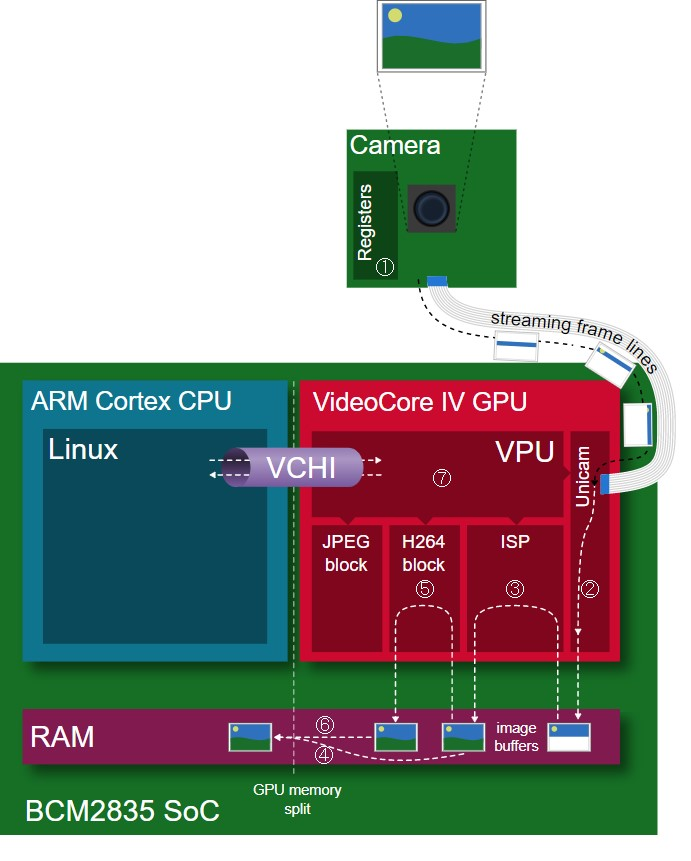
\includegraphics[scale=0.7]{images/рис_14.jpg}
  \caption{Передача изображения}
  \end{center}
\end{figure}

\begin{enumerate}
  \item Модуль камеры подключается к плате посредством пятнадцатижильного плоского шлефа длиной 15 см через последовательны интерфейс камеры (CSI), который имеет достаточную скорость передачи видеоданных в форматах до 1080p при 30 к/сек или 720p при 60 к/сек.
  \item А через интерфейс I$^2$C можно послыть команды управления камере.
  \item На плате также есть CSI-2 приемник, который также называют Unicam, через него и просходит принятие и отправка информации между "малинкой" и камерой.
  \item ISP (Image Signal Processor) конвертирует массив принятый байтов в изображение, которое уже способен воспринять человек. Этот компонент также взаимодействует с некторыми алгоритмами обработки изображения и сбора метаданных.
\end{enumerate}

На следующем рисунке более подробно демонстрируется связь интерфейсов платы и камеры.
\begin{figure}[h!]
  \begin{center}
    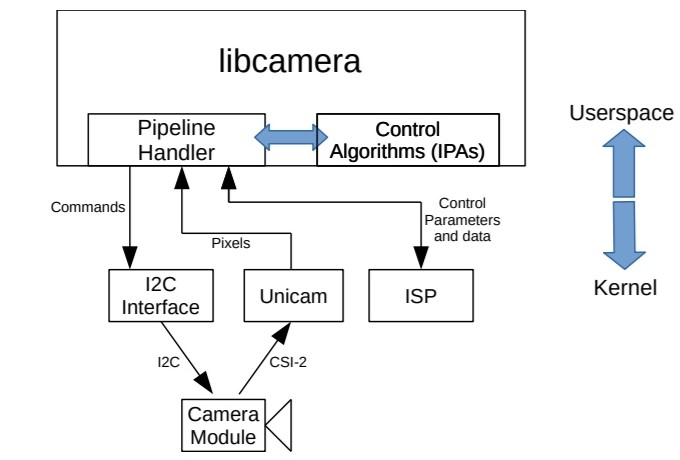
\includegraphics[scale=0.5]{images/рис_15.jpg}
  \caption{UNICAM}
  \end{center}
\end{figure}

\subsubsection{ПО для работы с камерой}
\begin{itemize}
  \item \verb|ffmpeg| - для кодеков,
  \item \verb|raspvid| - команда для записи видео,
  \item \verb|raspistill| - команда для захвата изображения (фото),
  \item \verb|PiCamera| - библиотека для Python. 
\end{itemize}

\section{Удаленное подключение к Raspberry Pi}
\noindent Для комфортной командной работы над проектом было решено настроить удаленный способ подключения к Raspberry Pi. Существует два распространенных способа удаленного управления:
\begin{itemize}
  \item Управление платой по протоколу SSH.
  \item Подключение к RPi с помощью VNC сервера.
\end{itemize}
\noindent Так как нам требовалось возможность работать в полноценном графическом режиме, был выбран второй способ.

\subsection{Настройка сервера}
Был установлен VNC сервер при помощи следующей команды:
\begin{verbatim}
  sudo apt-get install realvnc-vnc-server realvnc-vnc-viewer
\end{verbatim}
Затем в настройках RPi был включен VNC сервер:
\begin{figure}[h!]
  \begin{center}
    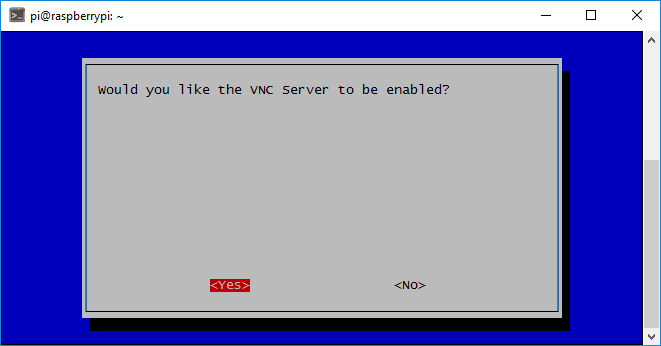
\includegraphics[scale=0.6]{images/image5.png}
  \caption{Включение VNC}
  \end{center}
\end{figure}

\noindent Запустили сервер при помощи команды \verb|vncserver|
В итоге мы увидели сообщение об удачном запуске сервера с IP-адресом и номером порта:
\begin{figure}[h!]
  \begin{center}
    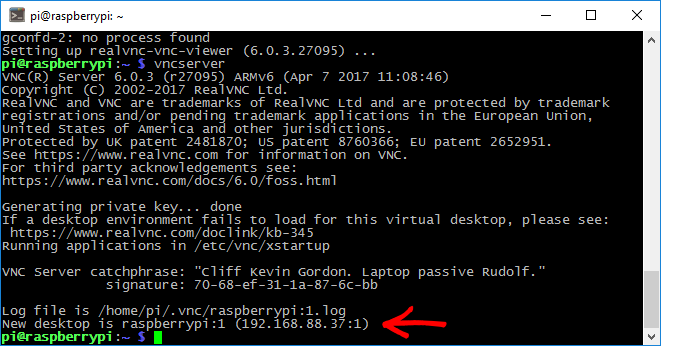
\includegraphics[scale=0.6]{images/image3.png}
  \caption{Номер порта}
  \end{center}
\end{figure}

\noindent Затем для удобства было решено прописать запуск VNC-сервера в автозагрузку Raspbian, чтобы не приходилось запускать его вручную после каждой перезагрузки.
Для этого мы перешли в папку с конфигурациями пользователя, создали директорию \verb|autostart| и в ней файл автозагрузки \verb|realvnc.desktop| и прописали следующее:
\begin{verbatim}
  [Desktop Entry]
  Type=Application
  Name=RealVNCServer
  Exec=vncserver :1
  StartupNotify=false
\end{verbatim}

\noindent Теперь при каждой загрузке графического интерфейса этот файл будет выполнять команду запуска VNC сервера.

\subsection{Настройка клиента}
На компьютеры участников проекта был скачан VNC-клиент VNC Viewer. Через File -> New connection создали подключение к Raspberry Pi, прописав его IP-адрес и порт, на котором прописан VNC-сервер.
\begin{figure}[h!]
  \begin{center}
    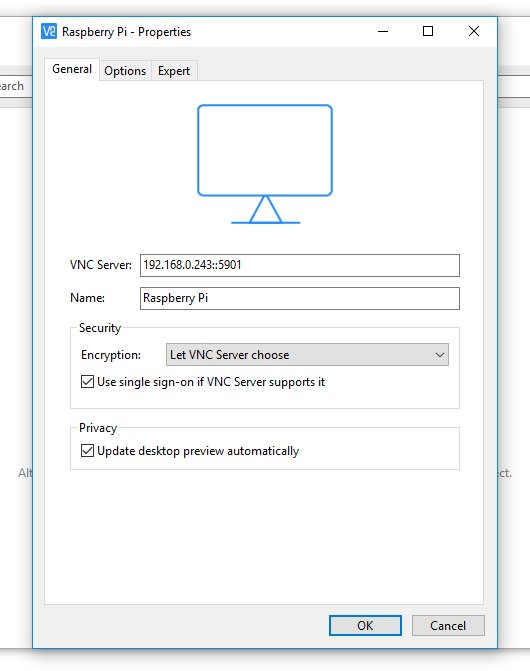
\includegraphics[scale=0.6]{images/image4.png}
  \caption{VNC Viewer}
  \end{center}
\end{figure}
\newpage
\noindent После ввода имени пользователя и пароля мы получили полный доступ к графическому интерфейсу RPi:
\begin{figure}[h!]
  \begin{center}
    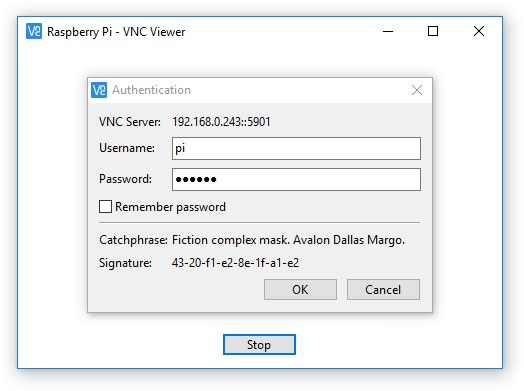
\includegraphics[scale=0.6]{images/image2.png}
  \caption{VNC Viewer авторизация}
  \end{center}
\end{figure}
\begin{figure}[h!]
  \begin{center}
    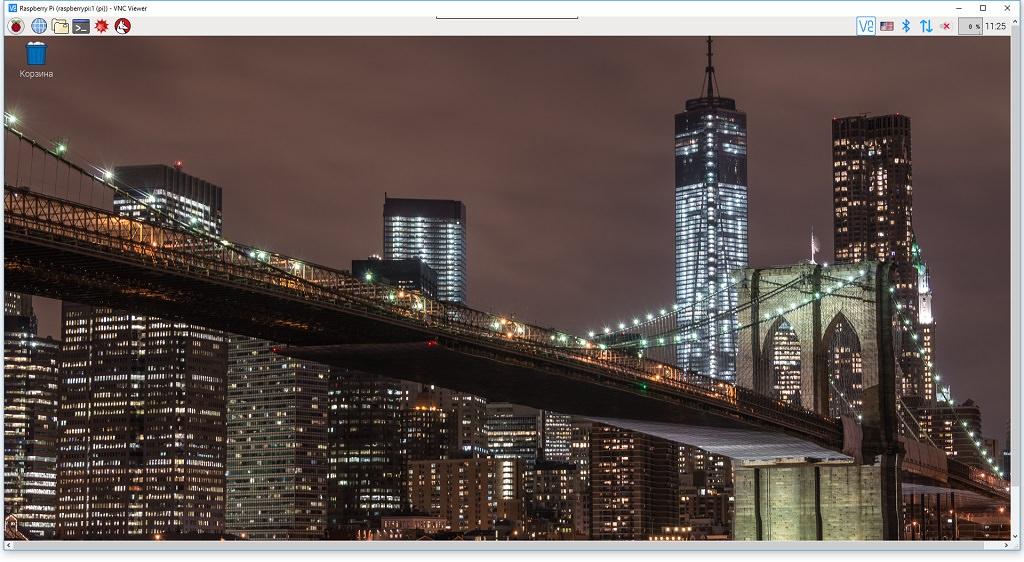
\includegraphics[scale=0.4]{images/image1.png}
  \caption{VNC Viewer успешное подключение}
  \end{center}
\end{figure}

\section{Программная реализация: \href{https://github.com/Yang-Pi/My-HomeCam-Security}{исходный код программы на GitHub}}
\noindent Как было сказано ранее, языком программирования был выбран \verb|Python|, а для решения задачи распознавания лиц была скачена библиотека \verb|OpenCV| и \verb|OpenCV-contrib|. \\

\noindent Рспознование лиц мы спроектировали на основе \textit{алгоритма Виолы-Джонса}, в основе которого лежат примитивы Хаары. Метод использует представление изображения в интегральном виде,
которое позволяет вычислять быстро, необходимые объекты, с помощью
признаков Хаара. Алгоритм применяет бустинг для выбора наиболее подходящих признаков для искомого объекта
на данной части заданного изображения. Метод использует классификатор,
на вход которого поступают все признаки, затем выдаётся результат «верно»
либо «ложь», то есть, принадлежит ли выделенный объект искомому классу
или нет. Для быстрого отбрасывания окон, где найден объект, используются
каскады признаков. Алгоритм распознает
черты лица под небольшим углом, примерно до 30 градусов. \\

\subsection{Описание схемы реализации}
\noindent Если обобщить, то наша программа состоит в последовавтельном вызове пяти процедур:
\begin{enumerate}
  \item Сбор данных (добавление нового объекта в базу данных).
  \item Обучение нейросети на основе обновленных данных.
  \item Распознавание (предсказание в процентах).
  \item Регистрация нажатия кнопки.
  \item Включение светодиода.
\end{enumerate}
А в целом схема система выглядит следующим образом (план-чертеж):
\begin{figure}[h!]
  \begin{center}
    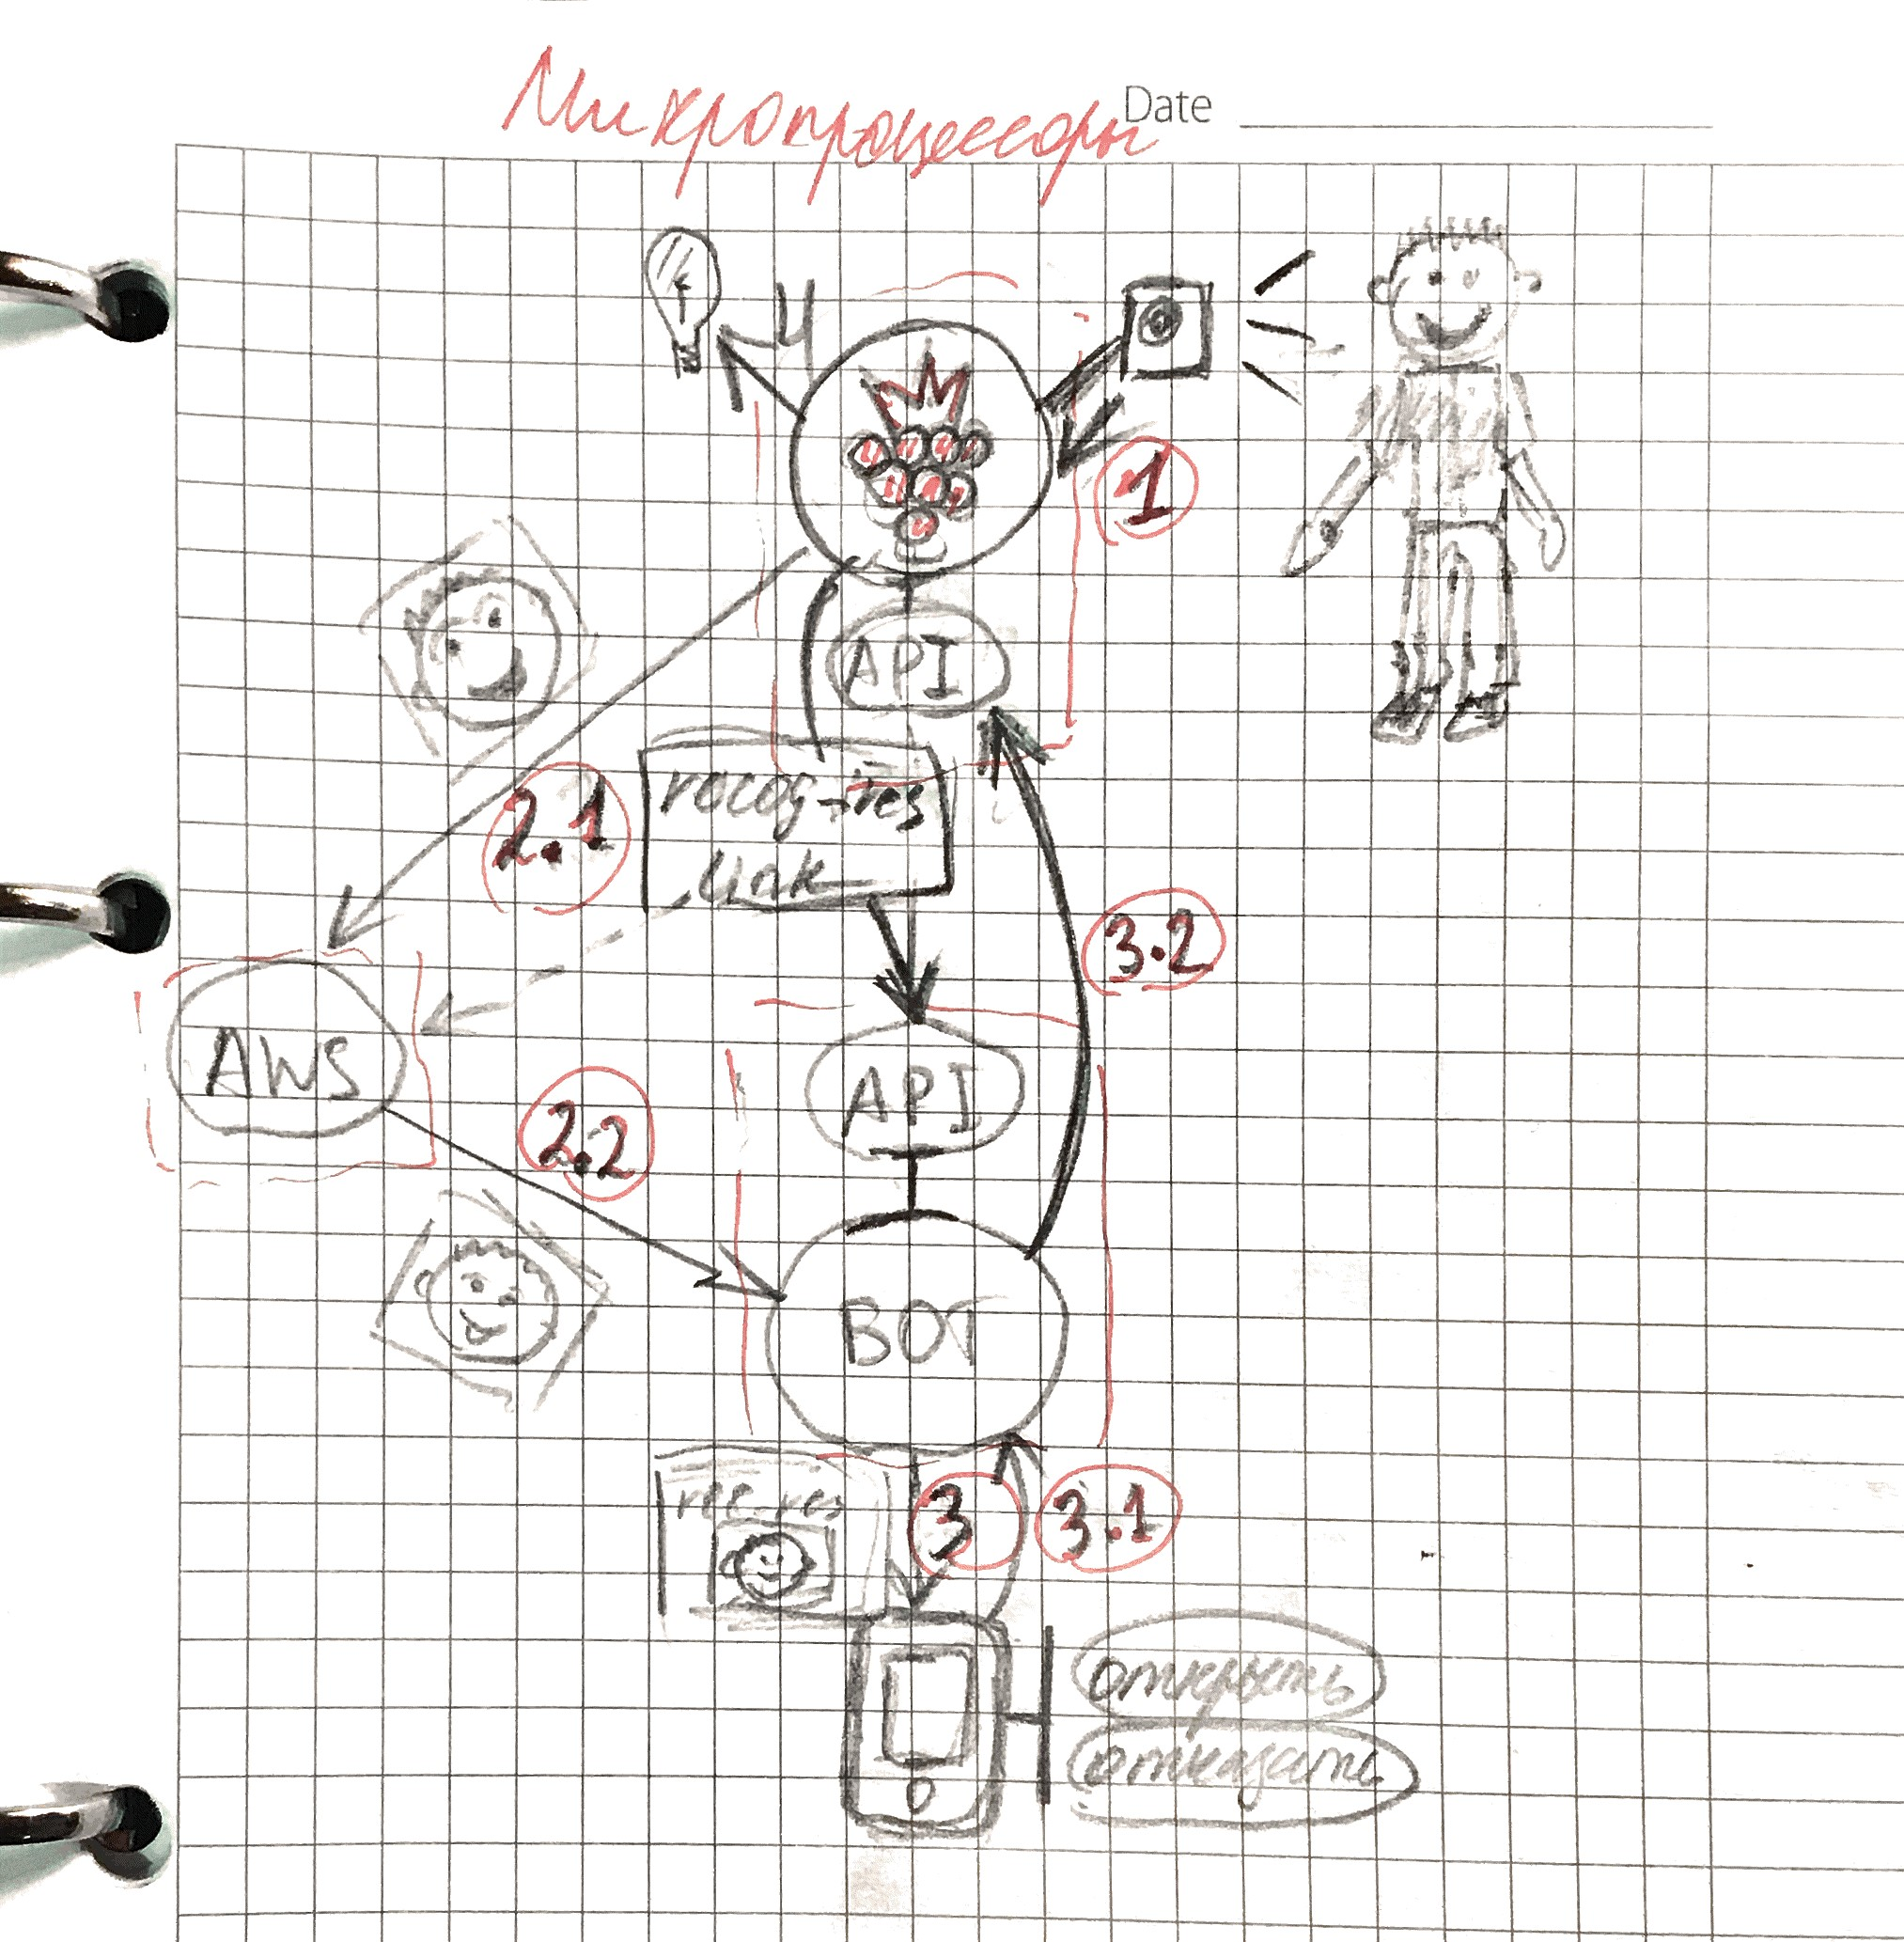
\includegraphics[scale=0.21]{images/рис_16.jpg}
  \caption{Схема программной реализации}
  \end{center}
\end{figure}
\newpage
\noindent Где
\begin{enumerate}
  \item Нажатие кнопки - работает 3-я и 4-я программы.
  \item Передача изображения и информации об объекте на нем хозяину.
  \item Ответ пользователя - работает 5-я программа.
\end{enumerate}
\noindent Регистрация нового гостя инициируется из бота, в этом случае срабатывают 1-я и 2-я программы по-порядку. \\
\subsubsection{Временная диаграмма активности компонентов системы}
\begin{figure}[h!]
  \begin{center}
    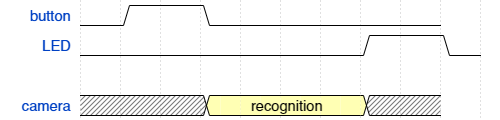
\includegraphics[scale=0.8]{images/рис_17.png}
  \caption{Активность компонентов}
  \end{center}
\end{figure}

\subsubsection{Функционал бота}
\begin{itemize}
  \item \textbf{Предоставление доступа}. При нажатии кнопки бот должен оповестить пользователя об этом и сообщить информацию вида: изображение нажавшего кнопку и результат распознавания. К сообщению прикреплены кнопки “Открыть” и “Не впускать”. Ответ отправляется в малину, которая включает соответствующий световой сигнал.
  \item \textbf{Регистрация человека}. Регистрируемый должен находиться перед камерой, чтобы было видно лицо. Далее владелец нажимает кнопку “Новый друг”, программа делает 300 снимков, нейросеть переобучается, владелец вводит имя друга, которое вместе с id пользователя для нейронки заносятся в базу данных.
  \item \textit{Включить трансляцию}. В боте есть кнопка на клавиатуре (и команда) ”Online”. При нажатии предоставляется ссылке, перейдя по которой открывается трансляция в прямом эфире с камеры. Дополнительно можно сделать пароль для пользователя, чтобы только он мог смотреть. После необходимо завершить трансляцию. Или же она прервется другими операциями.
\end{itemize}

\noindent В реализации бота использовался следующий технологический стек:
\begin{itemize}
  \item Python + Django
  \item Ngrok
  \item Celery + Redis
  \item TelegramBot API
\end{itemize}

\section{Демонасрация работы системы}
\href{https://drive.google.com/drive/u/0/folders/17Fis1vASnBp3RG1X3LoO70RmMCvE8m6c}{Все видео, начиная с этапов тестирования отдельных компонентов}
\begin{figure}[h!]
  \begin{center}
    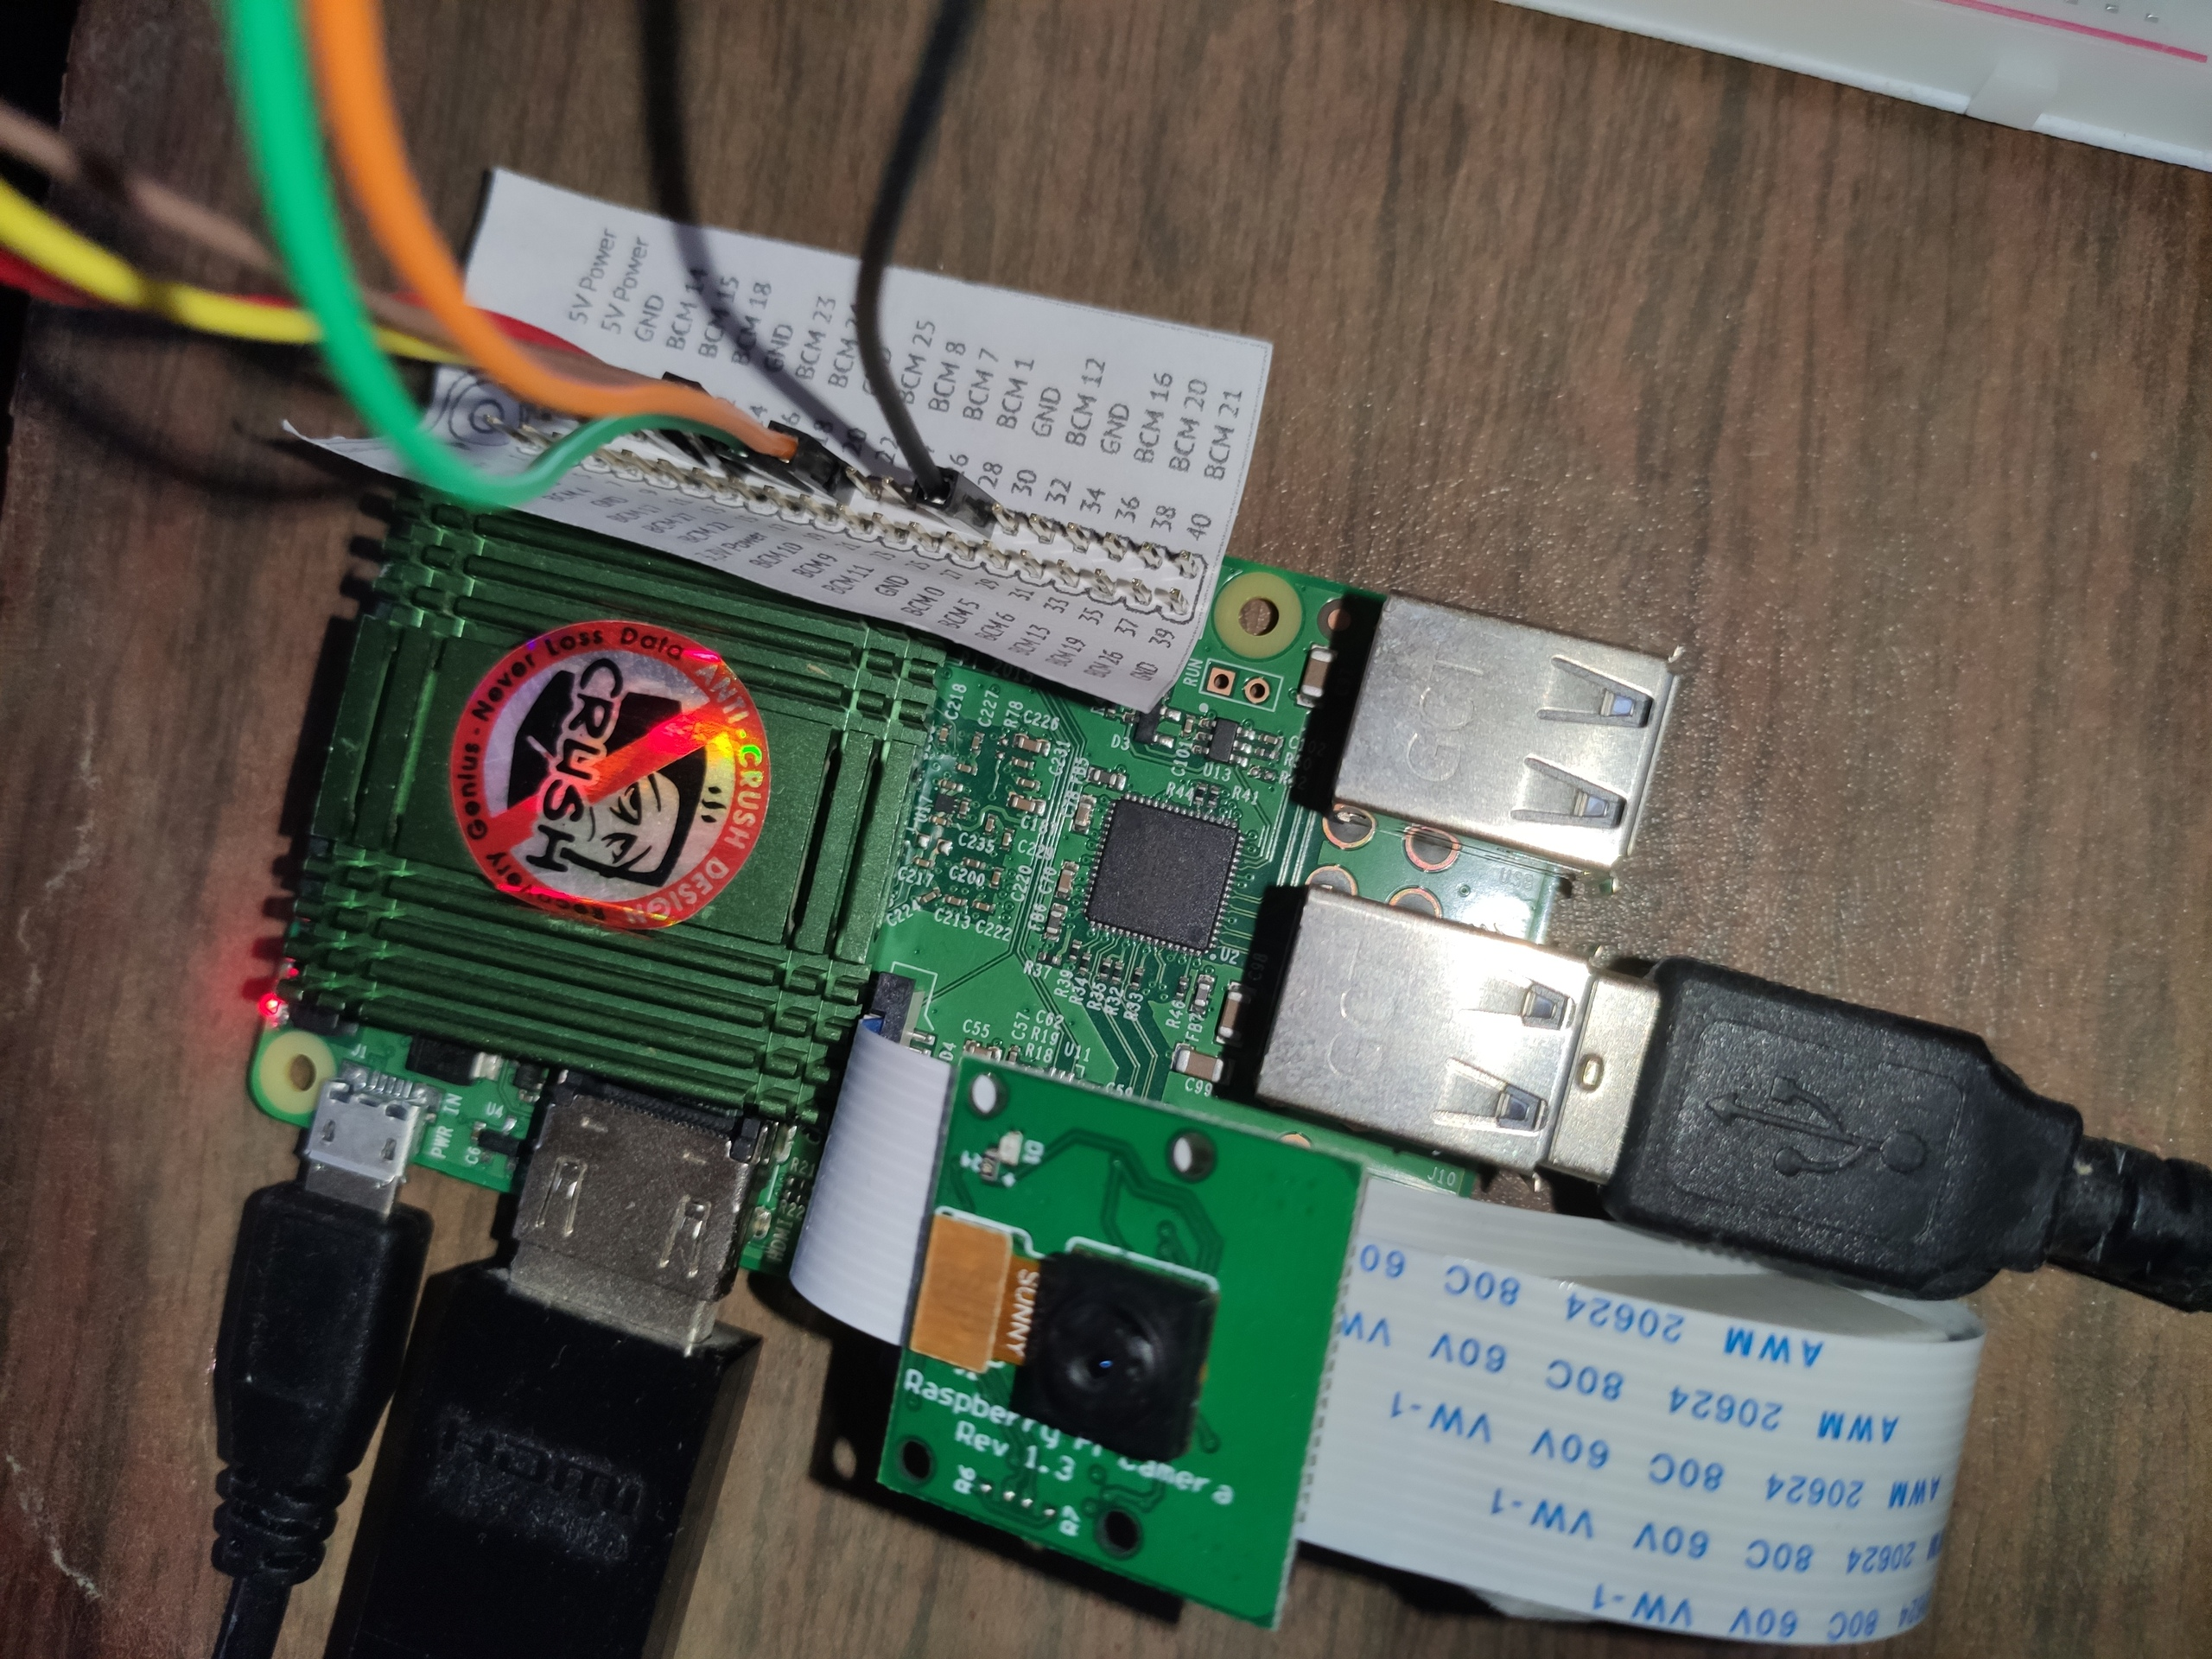
\includegraphics[scale=0.15]{images/апп_1.jpg}
  \caption{Наша плата и камера}
  \end{center}
\end{figure}
\begin{figure}[h!]
  \begin{center}
    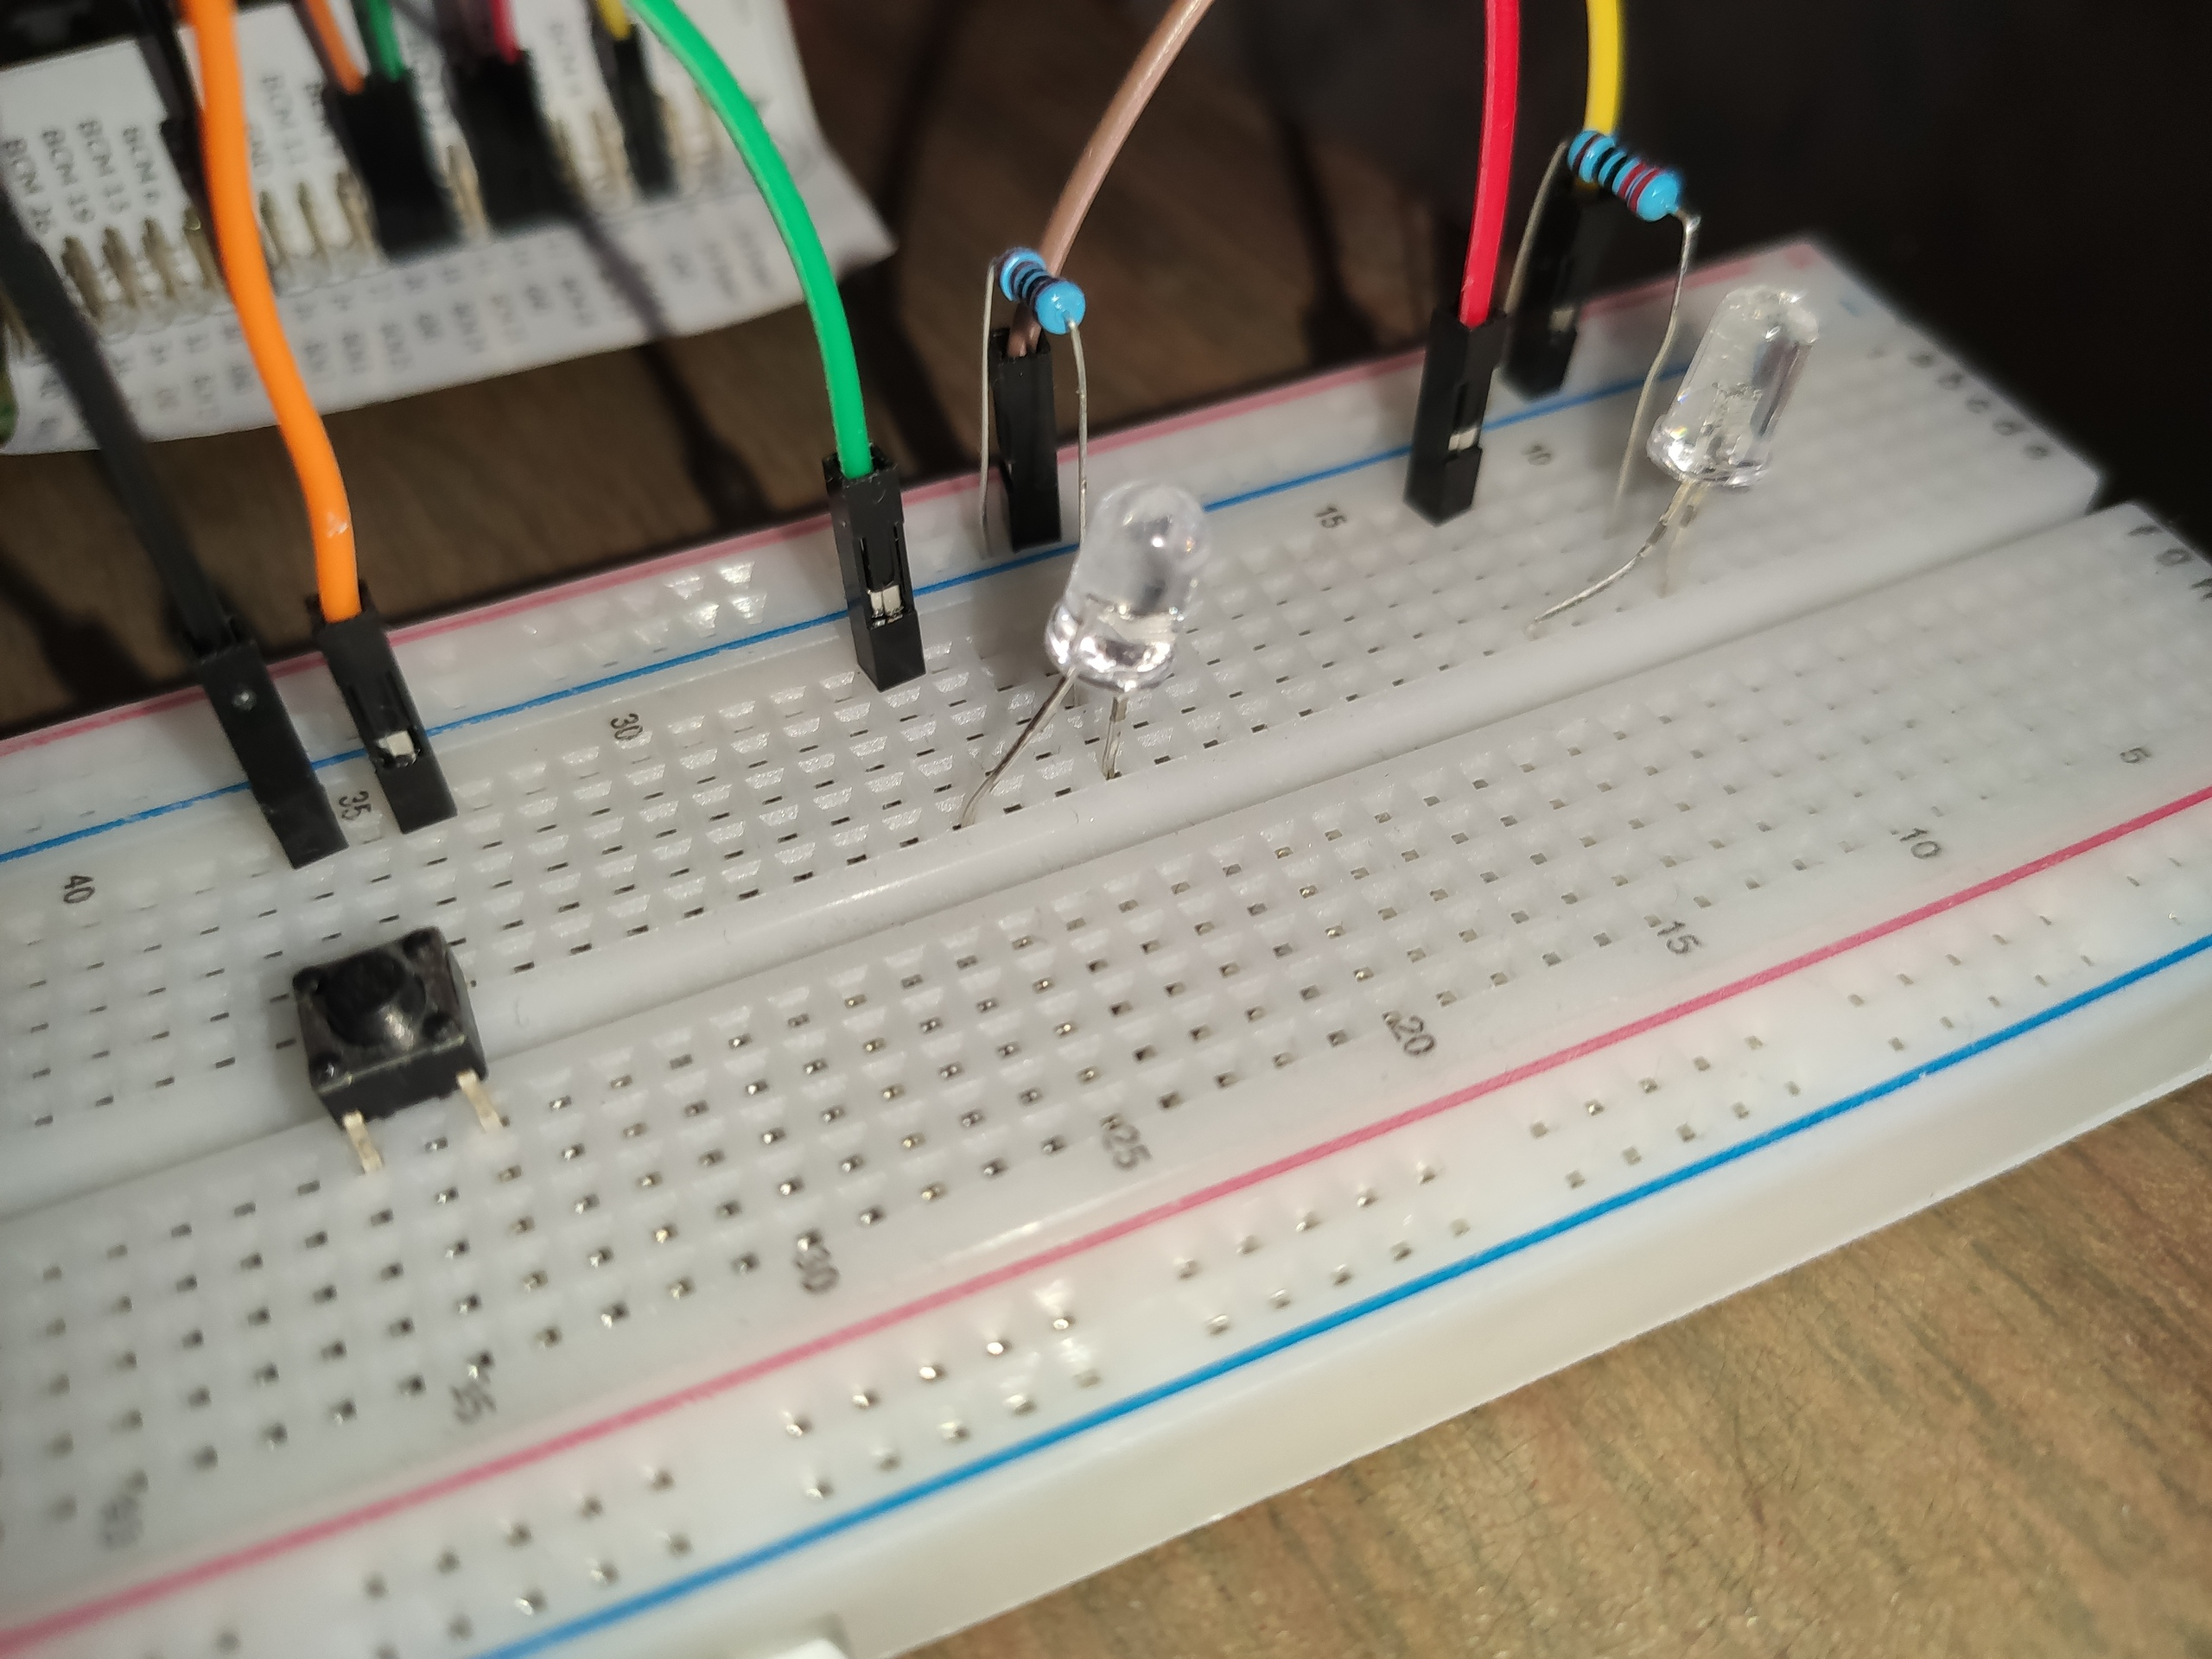
\includegraphics[scale=0.15]{images/апп_2.jpg}
  \caption{Наши кнопки и светодиоды}
  \end{center}
\end{figure}


\section{Вывод}
В ходе работы по реализации системы контроля входа в умном доме мы исследовали возможности микрокомпьютера Raspberry Pi 3 Model B, на котором установлен процессор ARM Cortex-A53, подключали к плате различные перефирийные устройства, а именно камеру, кнопку и два светодиода, и следили за их правильным функционированием, контролируя процессы через различные интерфейсов (GPIO, CSI, I$^2$C).

\end{document}